% Dokument:
\documentclass[a4paper,10pt,twocolumn]{article}
\usepackage[utf8]{inputenc}
%\usepackage[norsk]{babel}
\usepackage{hyperref}

% Formatering:
\usepackage{geometry,amsthm,blindtext}
\setlength{\parindent}{0mm}
\setlength{\parskip}{1.8mm}
% Symboler
\usepackage[geometry]{ifsym}
% Matematikk:
\usepackage{amsmath,mathtools,amsfonts,xparse,physics,esint,mathrsfs,nicefrac,siunitx}
% Kode:
\usepackage{verbatim,listings,algpseudocode}
% Tekst:
\usepackage{textcomp,varioref,enumerate,bbold}
% Figurer:
\usepackage{graphicx,subcaption,float,dcolumn,multirow}
%\usepackage[section]{placeins}
% Farge:
\usepackage{xcolor}

% Dcolumn-kolonner
\newcolumntype{,}{D{,}{{,}}{2}}
\newcolumntype{=}{D{=}{=}{-1}}
\newcolumntype{.}{D{.}{{.}}{2}}
\newcolumntype{C}{>{$}c<{$}}

% Listings-Instillinger
	\lstset{
	% Språk
	language=c++,
	% Farge
	backgroundcolor=	\color[rgb]{0.9,0.9,0.9},
	keywordstyle=		\color[rgb]{0,0,1},
        	commentstyle=		\color[rgb]{0.133,0.545,0.133},
        	stringstyle=		\color[rgb]{0.627,0.126,0.941},
	numberstyle=\tiny	\color[rgb]{0.5,0.5,0.5},
        	rulecolor=			\color{black},
	% Tekst:
	basicstyle=\scriptsize,
	showspaces=false,
	showstringspaces=false,
	showtabs=false,
	% Spesialtegn
	extendedchars=true,
        	literate=	{æ}{{\ae}}1 	{ø}{{\o}}1 		{å}{{\r a}}1 
		  	{≤}{{$\leq$}}1 	{≥}{{$\geq}}1	{–}{{$-$}}1		{~}{{\tiny{$\sim$}}}1,
        	% Format
	frame=single,
	aboveskip={1.5\baselineskip},
	breaklines=true,
	columns=fixed,
	numbers=left,
	numbersep=5pt,
	stepnumber=1,
	tabsize=4, 
	% ... 
        	upquote=true,
        	prebreak = \raisebox{0ex}[0ex][0ex]{\ensuremath{\hookleftarrow}},
        	identifierstyle=\ttfamily
        	}
	
% Nummerering:
%\renewcommand{\thesection}{\arabic{section}}		% Nummer i "section"
%\renewcommand{\thessubection}\arabic{subsection}}	% Nummer i "subsection"
%\renewcommand{\thesection}{\alph{section}}			% Bokstaver i ''section''
%\renewcommand{\thesubsection}{\alph{subsection}}	% Bokstaver i ''subsection''

% Egendefinerte kommandoer:
	% Snarveier
	\newcommand*{\eqset}[1]{\begin{dcases}#1\end{dcases}}
	\newcommand*{\Qfig}[3]{\begin{figure}[ht]	\centering \includegraphics[#2]{#1} \caption{#3} \end{figure} }
	% Tegn
	\newcommand{\point}{\varointclockwise}	% integral med klokken
	\newcommand{\noint}{\ointctrclockwise}	% integral mot klokken
	\newcommand{\ee}[1]{\!\times\!\!10^{#1}} 	% 10 i #1-te
	\newcommand{\un}[1]{\,\si{#1}}		% enheter
	\newcommand{\e}[1]{\mathrm{e}^{#1}}	% exp()
	\newcommand{\ci}{\dot{\iota\!\:}}		% kompleks i
	% misc
	\newcommand{\note}[1]{{\color{red}\quad[$\backslash!/$: #1]}}	% notater for dokument under arbeid
	\newlength{\txtsz}\makeatletter\setlength{\txtsz}{\f@size pt}\makeatother
	\newcommand{\insubsec}[1]{\par{\bf #1}}

% Åpning:
\title{Building a model for the solar system using ordinary differential equations}
\author{Johannes Sørby Heines}


% START
\begin{document}

\twocolumn[
\begin{@twocolumnfalse}
\maketitle
\begin{abstract}
We developed a program to simulate a system of objects interacting via classical gravity, using different differential equation solver algorithms. The program was applied to the Earth-Sun system, showing a relative increase of 67\% in energy and 70\% in negative angular momentum for the Forward Euler algorithm, and conservation with the Euler-Cromer and velocity Verlet algorithms. The latter was found to be the most accurate.  
The program was also used to show the effect of Jupiter on the Earth's orbit, and to simulate all planets in the solar system, and Pluto. 

\end{abstract}
\end{@twocolumnfalse}
]

\section*{Introduction}
The motion of celestial objects is usually determined only by the force of gravity. Since gravity has infinite range, every body in a system interacts with every other body in that system. This makes analytical calculations impossible in all but a very few highly specific cases. 
The goal of this project was to implement a program to simulate the motion of objects in space numerically, and apply it to the planets in the Solar system.

The next section describes our model of the solar system, outlines the numerical algorithms for solving it and their implementation, and summarizes the structure of the program.
We then compare the algorithms for a two-body problem, study a three-body problem and apply the program to the solar system. Finally we discuss shortcomings of the program and suggest improvements. 


%
%
%
\section*{Theoretical models and implementation}
All code can be found, along with unit tests and benchmarks at \url{https://github.com/johashei/ComputationalPhysics/tree/master/doc/Projects/2020/Project3/code}.

\subsection*{The solar system}
The bodies in the solar system can be modeled as point particles interacting gravitationally. 
The newtonian gravitational force between two bodies of mass $m_1$ and $m_2$ is
\[
F = G\frac{m_1m_2}{r^2},
\]
where $G$ is the gravitational constant and $r$ is the distance between the bodies.

In reality the gravitational interaction is described by the general theory of relativity. However, for the solar system, the newtonian model is a good approximation for all planets except Mercury. Indeed, observed perihelion precession of Mercury is $43\un{\arcsecond}$ per century larger than can be explained by classical effects, such as the gravitational force from the other planets \cite{labtext}.

The effect of general relativity can be accounted for by adding a correction term to the force, giving \cite{labtext}
\[
F = G\frac{m_\odot m_\text{Mercury}}{r^2}\qty[1 + \frac{3l^3}{r^2c^2}],
\]
where $m_\odot$ is the mass of the Sun, $m_\text{Mercury}$ is the mass of Mercury, $l = \abs{\vec{r}\cross\vec{v}}$ is Mercury's orbital angular momentum and $c$ is the speed of light in vacuum.

We began by creating a program for simulating the solar solar system classically. 
And then attempted to study the effect of the general relativity correction above on Mercury.

Measuring the effect of the general relativity correction requires the a time resolution such that the perihelion precession for the classical case is more than one order of magnitude smaller than what is expected with the relativistic correction. In other words, it must be of the order of $10^{-2}\un{\arcsecond\cdot yr^{-1}}$ or smaller.


\subsection*{Numerical integration methods}
The movement of a body of mass $m$ under the influence of a conservative force $\vec{F}$ is given by the second order differential equation
\[
\dv[2]{\vec{r}}{t} = \frac{\vec{F}}{m}.
\] 
In the case of gravity, the force depends on the position and mass of all bodies in the system. There are multiple ways of solving such a problem numerically. We studied Forward Euler, Euler-Cromer and velocity Verlet. They all separate the equation into two first order differential equations, and approximate these by Taylor expansions. 
\begin{align*}
x(t\pm h) &= x(t) \pm h\dot{x}(t) + \frac{h^2}{2}\ddot{x}(t) \pm \order{h^3} \\
\dot{x}(t\pm h) &= \dot{x}(t) \pm h\ddot{x}(t)  + \frac{h^2}{2}x^{(3)}(t) \pm \order{h^3}
\end{align*}
The Forward Euler method uses only a first order Taylor expansion. 
For $M$ objects and $N$ time steps, the algorithm is
\begin{algorithmic}
\For{i = 0:N}
\For{j = 0:M}
\State $a_{i,j} = a(\vec{x}_i,j)$
\State $v_{i+1,j} = v_{i,j} + h\cdot a_{i,j}$
\State $x_{i+1,j} = x_{i,j} + h\cdot v_{i,j}$
\EndFor
\EndFor
\end{algorithmic}
Here $v=\dot{x}$ is the velocity, $a=\ddot{x}$ is acceleration, and $\vec{x}_i$ contains the positions of all objects at time point $i$. 

While this algorithm is very simple to implement, the error in each time step is $\order{h^2}$, which over $N\sim 1/h$ time steps gives a global error $\order{h}$. In addition, it can be shown that this algorithm does not conserve the energy of the system \cite{lecture}. 

This last point is addressed by the Euler-Cromer algorithm. By changing the second expression to $x_{i+1,j} = x_{i,j} + h\cdot v_{i+1,j}$, the algorithm becomes energy conserving \cite{lecture}. The global error, however, remains the same. 

The velocity Verlet method uses second order Taylor approximations of $x$ and $v$, with a first order Taylor approximation   of $\ddot{v}$. The algorithm is \cite{lecture}
\begin{algorithmic}
\For{i=0:N}
\For{j=0:M}
\State $x_{i+1,j} = x_{i,j} + h\cdot v_{i,j} + \frac{h^2}{2} a_{i,j}$
\EndFor
\For{j=0:M}
\State $a_{i+1,j} = a(\vec{x}_{i+1},j)$
\EndFor
\For{j=0:M}
\State $v_{i+1,j} = v_{i,j} + \frac{h}{2}(a_{i+1,j} + a_{i,j})$
\EndFor
\EndFor
\end{algorithmic}
Note here that the position of every body must be calculated before calculating the velocities. In this method, the local error in each iteration is $\order{h^3}$, giving a global error of $\order{h^2}$. It can also be shown that this algorithm conserves energy \cite{lecture}.


Since no external force is acting on the solar system, the total energy $E$ and angular momentum $\vec{L}$ are conserved. Calculating the change of these quantities over the course of the simulation is therefore a good way of comparing the accuracy of different algorithms.

\begin{comment}
The Euler algorithms and the velocity Verlet algorithm differ greatly in number of floating point operations (FLOPs). For Euler and Euler-Cromer, each iteration takes $4+A$ FLOPs, where $A$ is the number of flops used when calculating the acceleration. This number depends on the system, but is the same in all algorithms. The total number of FLOPs required is then $(4+A)MN$. 
In the velocity Verlet algorithm, the constants $h/2$ and $h^2/2$ can be calculated outside the loop. The total number of FLOPs is then $(4+A+3)MN$.
Because we store the position and velocity values in a pseudo-multidimensional array, our program requires an additional $(2M+1)N$ FLOPs to calculate the indices for each loop. This bring the total up to $[(6+A)M+1]N$ FLOPs for Euler and $[(11+A)M+2]N$ FLOPs for velocity Verlet.
\end{comment}

The differences between the three algorithms were studied in a two-body system, with the Earth in a circular orbit around the sun. 
Here we chose a small number of time steps ($10^4$ over 10 years) in order to see the differences clearly. 
We then added Jupiter, also in a circular orbit, and observed the effects of changing Jupiter's mass from $1.9\ee{27}\un{kg} \approx M_\odot/1000$ to $1.9\ee{30}\un{kg} \approx M_\odot$.


\subsection*{Object orientation}

Our goal was to write a general program which could simulate any three dimensional system of point particles. 
The first step was to create a class for defining a point particle. An instance of the PhysicsObject class contains position and velocity vectors and mass. The vectors are defined with the vec3 class, which adds vector operations to the C++ vector class. 
The PhysicsObject class is completely inlined, allowing it to be accessed within vectorized loops. 

The simulation of the system is done by the PhysicsSimulator class. Since the numerical integration methods studied here, that is Euler, Euler-Cromer and velocity Verlet, require few lines to implements, but access to multiple class variables, we chose against creating a dedicated solver class.

The calculations of energy an angular momentum are done in a separate Tests class. This class is initialized with a reference to a PhysicsSimulator instance. It then calculates and compare $E$ and $\vec{L}$ of the first and final time. 

%
%
%
\section*{Results}
%With $\rho_N = 30$ and $N=
\begin{figure*}[b]
	\centering
	\begin{subfigure}{.33\textwidth}
		\centering
		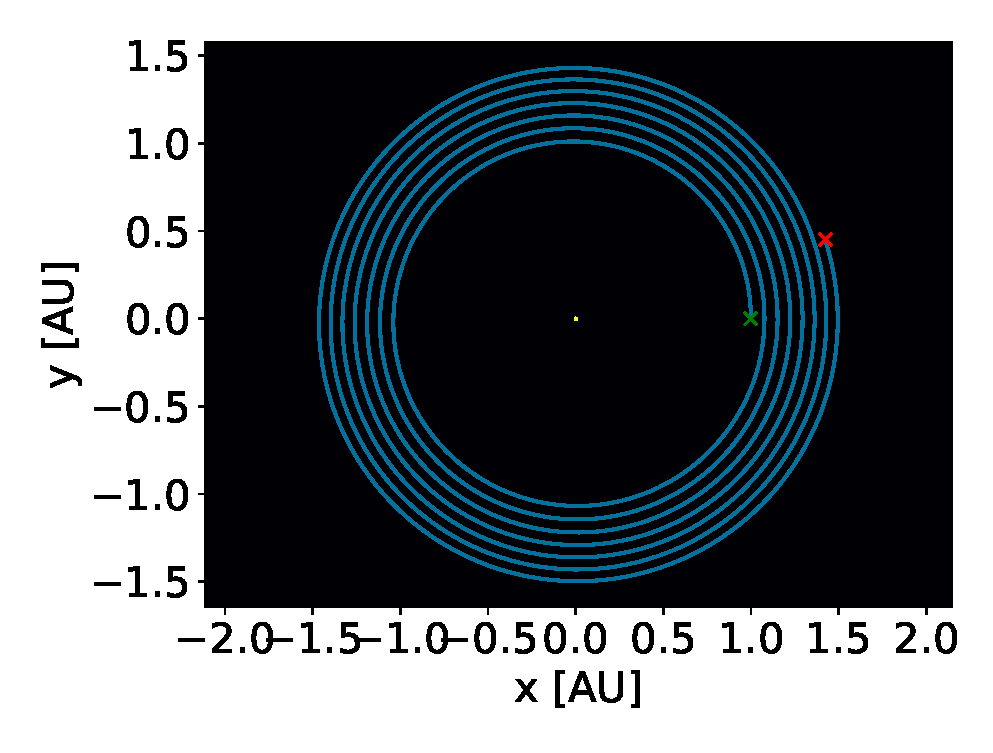
\includegraphics[width=\linewidth]{es10e4.eps}
		\caption{Forward Euler method\\
	 		$
			\Delta L = -4.23\ee{-6} \un{M_\odot AU^2yr^{-1}}
			\\\Delta E = 1.97\ee{-5} \un{M_\odot AU^2 yr^{-2}}
			$}
	\end{subfigure}%
	\begin{subfigure}{.33\textwidth}
		\centering
		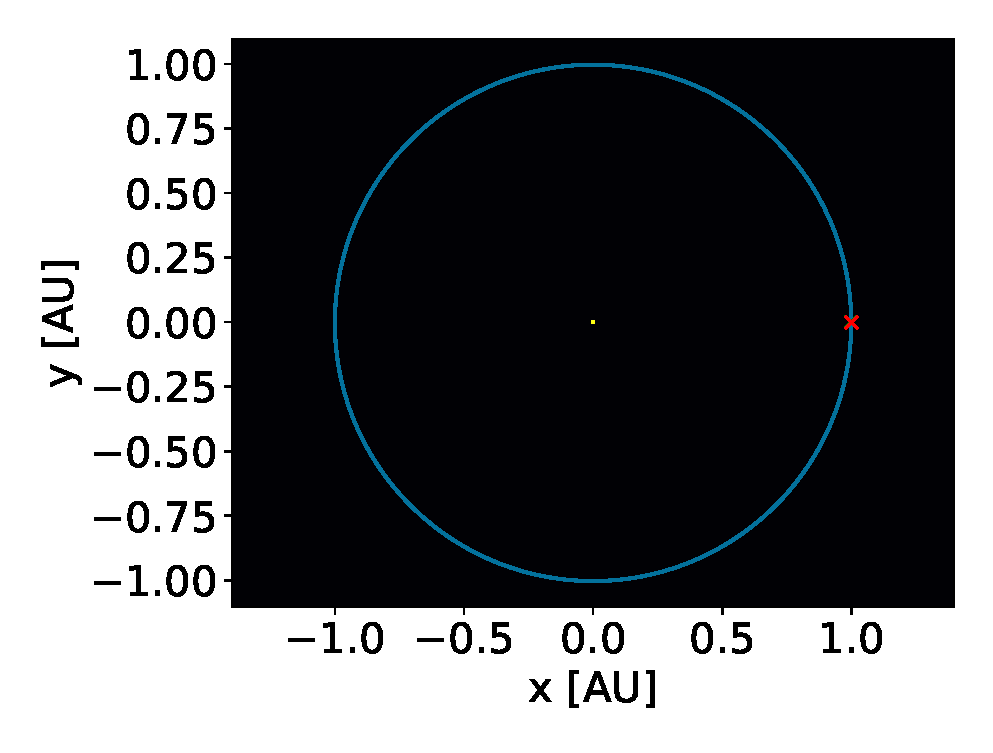
\includegraphics[width=\linewidth]{es10ec4.eps}
		\caption{Euler-Cromer method\\
			$
			\Delta L = 1.12\ee{-19} \un{M_\odot AU^2yr^{-1}}
			\\\Delta E = 1.19\ee{-15} \un{M_\odot AU^2 yr^{-2}}
			$}
	\end{subfigure}%
	\begin{subfigure}{.33\textwidth}
		 \centering
		 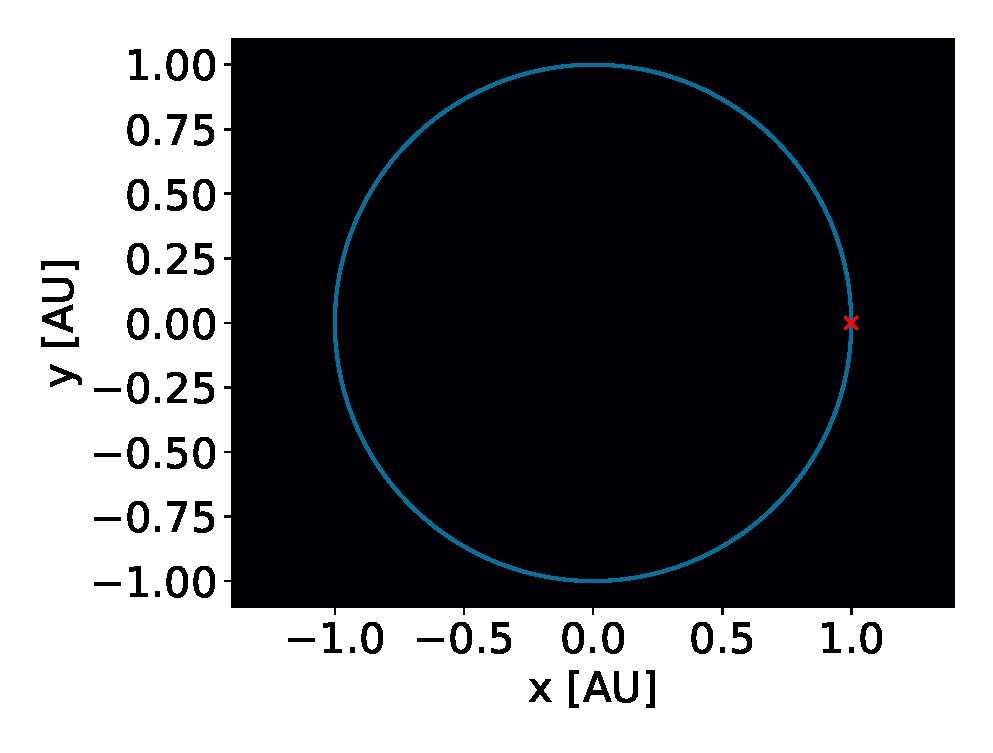
\includegraphics[width=\linewidth]{se10vv4.eps}
		 \caption{Velocity Verlet method\\
		 $
		 \Delta L = -7.12\ee{-20} \un{M_\odot AU^2yr^{-1}}
		 \\\Delta E = 4.13\ee{-19} \un{M_\odot AU^2 yr^{-2}}
		 $}
	\end{subfigure}
	\caption{Plots of the Sun-Earth system obtained with the different algorithms. All simulations used $10^4$ time steps over 10 years. The start and end points are marked by a green and a red cross ($\cross$), respectively. The total change in angular momentum $L$ and energy $E$ are given in each case.}
	\label{fig:compare}
\end{figure*}

Most of the effect of the algorithms are best illustrated using only one planet. 
Figure \ref{fig:compare} shows the result of simulating the orbit of the Earth over 10 years with the three algorithms. The Earth has been given a circular orbit, so the total energy of the system is
\begin{align}
E &= \frac{1}{2}M_\oplus v^2 - G\frac{M_\odot M_\oplus}{d^2}	\nonumber
%\\&= \frac{1}{2}3\ee{-6}(2\pi)^2 - 4\pi^2\frac{3\ee{-6}}{1}
\\&= 5.92\ee{-5} \un{M_\odot AU^2 yr^{-2}},	\label{eq:E}
\end{align}
and the total angular momentum
\begin{align}
\vec{L} &= M_\oplus\vec{r}\cross\vec{v}	\nonumber
\\&= [0,0,-1.88\ee{-5}] \un{M_\odot AU^2 yr^{-1}}. \label{eq:L}
\end{align}
Here $\vec{r}$ and $\vec{v}$ are the position and velocity of the Earth relative to the Sun, respectively.

Figure \ref{fig:esj} shows the effect of introducing a third object to the system. 

\begin{figure*}
	\centering
	\begin{subfigure}{.5\textwidth}
		\centering
		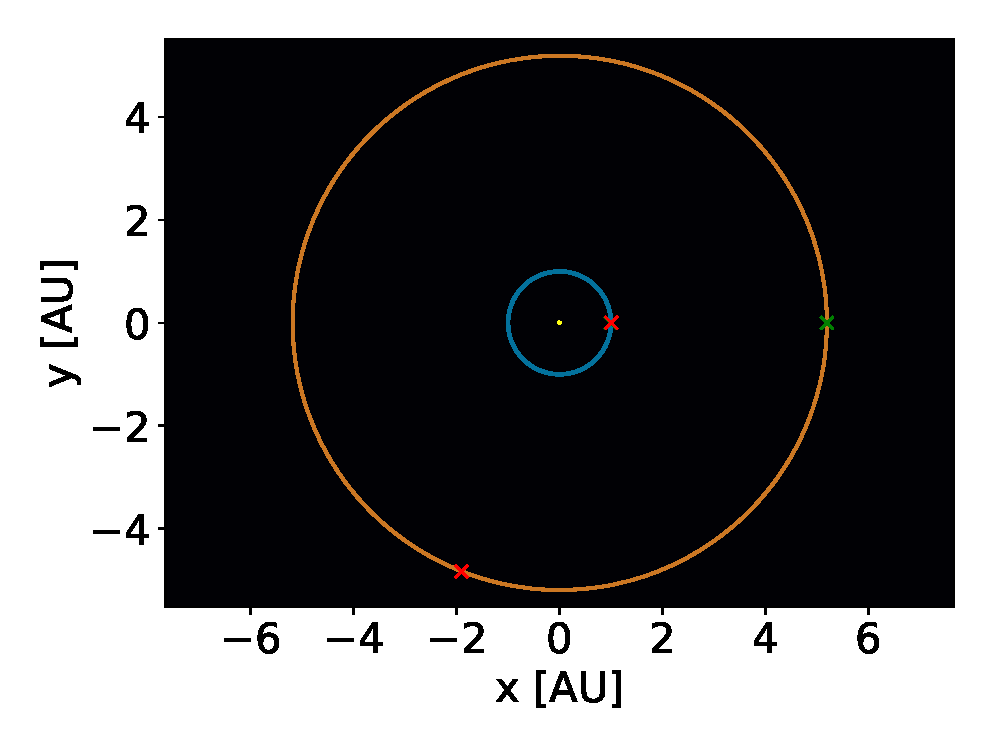
\includegraphics[width=\linewidth]{esj20vv7.eps}
		\caption{$M_\text{Jupiter} \approx M_\odot/1000$}
	\end{subfigure}%
	\begin{subfigure}{.5\textwidth}
		\centering
		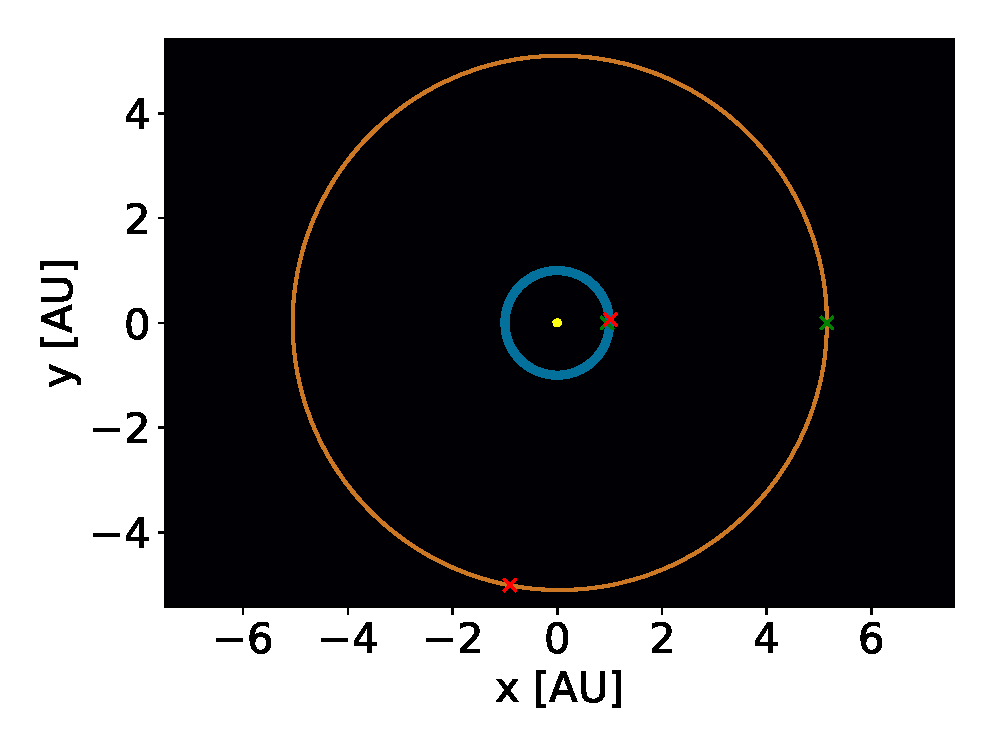
\includegraphics[width=\linewidth]{esjx1020vv7.eps}
		\caption{$M_\text{Jupiter} \approx M_\odot/100$}
	\end{subfigure}%
	\newline%
	\begin{subfigure}{.5\textwidth}
		\centering
		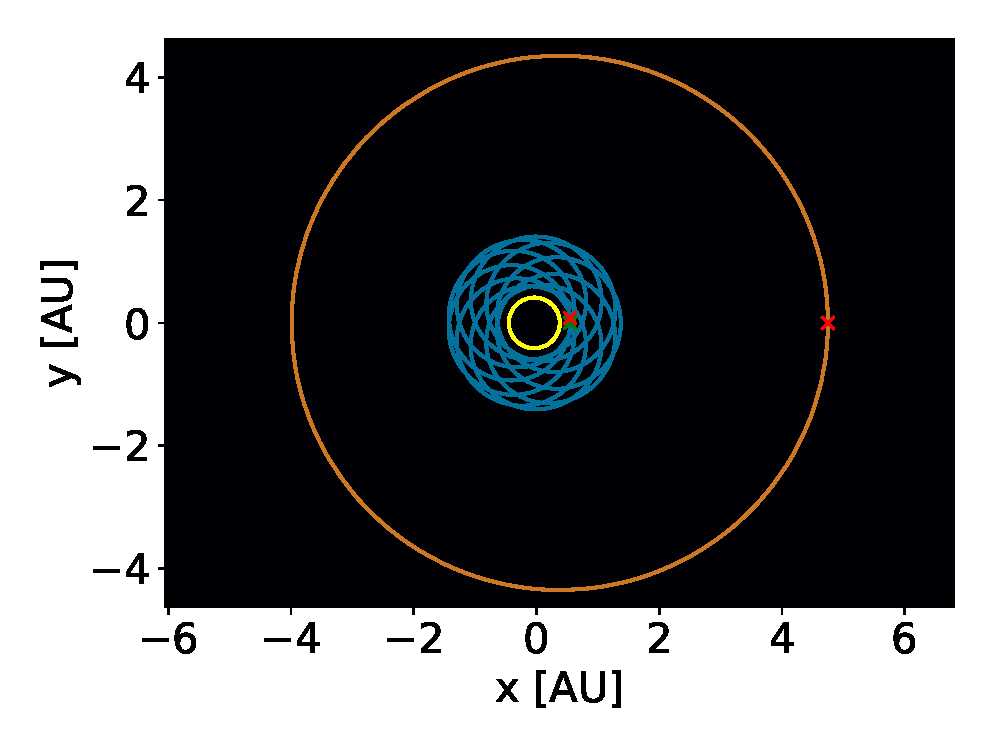
\includegraphics[width=\linewidth]{esjx10010vv7.eps}
		\caption{$M_\text{Jupiter} \approx M_\odot/10$}
		\label{fig:esj10}
	\end{subfigure}%
	\begin{subfigure}{.5\textwidth}
		 \centering
		 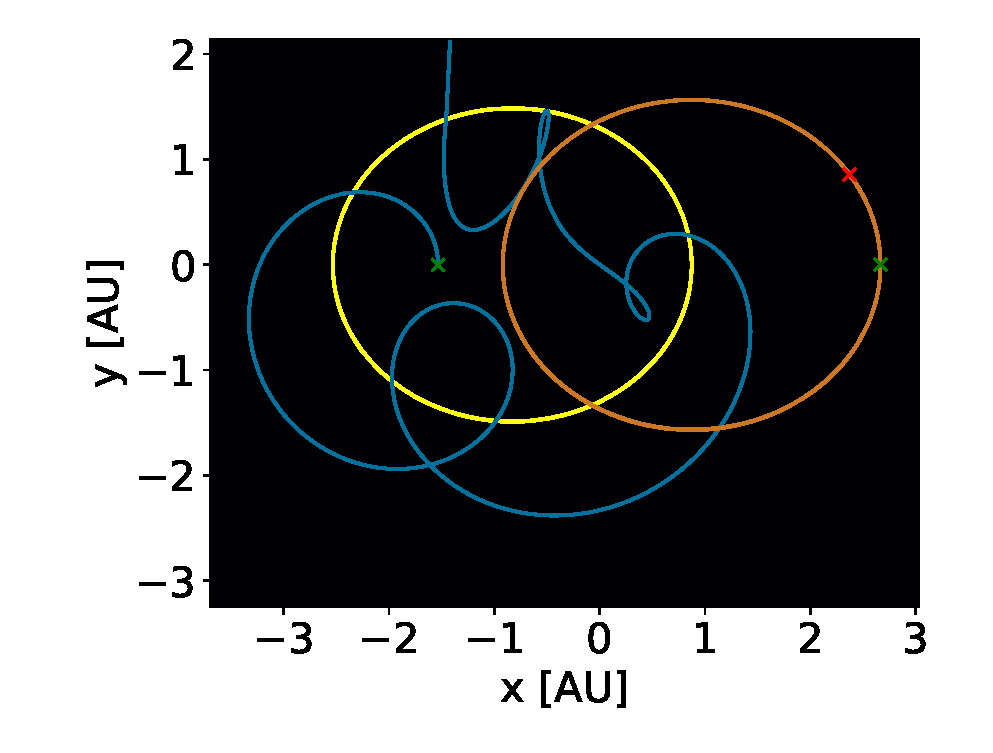
\includegraphics[width=\linewidth]{esjx100010vv7.eps}
		 \caption{$M_\text{Jupiter} \approx M_\odot$}
		 \label{fig:esj1}
	\end{subfigure}
	\caption{Plots of the Sun-Earth-Jupiter system for different masses of Jupiter, obtained with the velocity Verlet method with $10^7$ time steps. In the first two cases, energy and angular momentum are conserved. In the last, angular momentum is conserved, but $\Delta E = 0.60\un{M_\odot AU^2 yr^{-2}}$}
	\label{fig:esj}
\end{figure*}


\begin{figure*}
	\centering
	\begin{subfigure}{.5\textwidth}
		\centering
		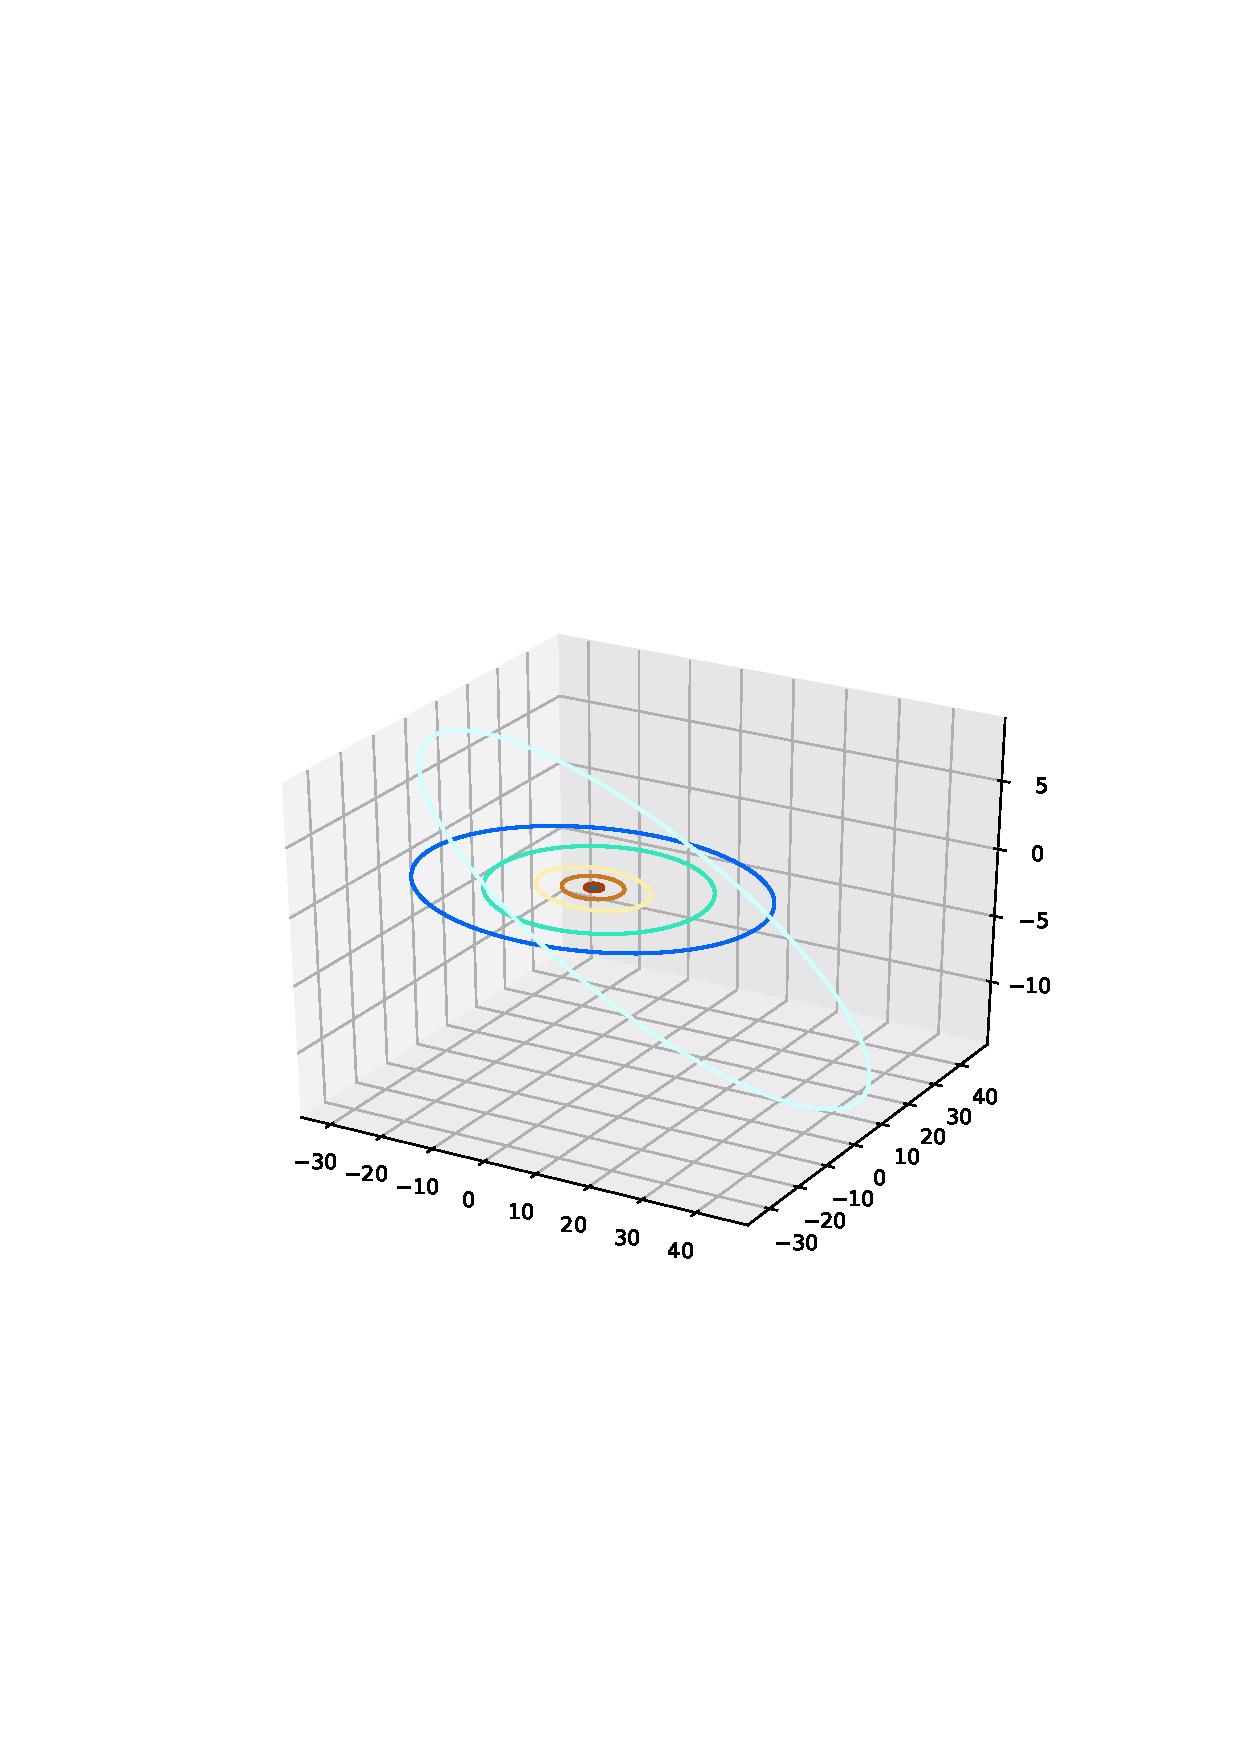
\includegraphics[width=\linewidth]{sol250vv73d.pdf}
		\caption{3D}
	\end{subfigure}%
	\begin{subfigure}{.5\textwidth}
		\centering
		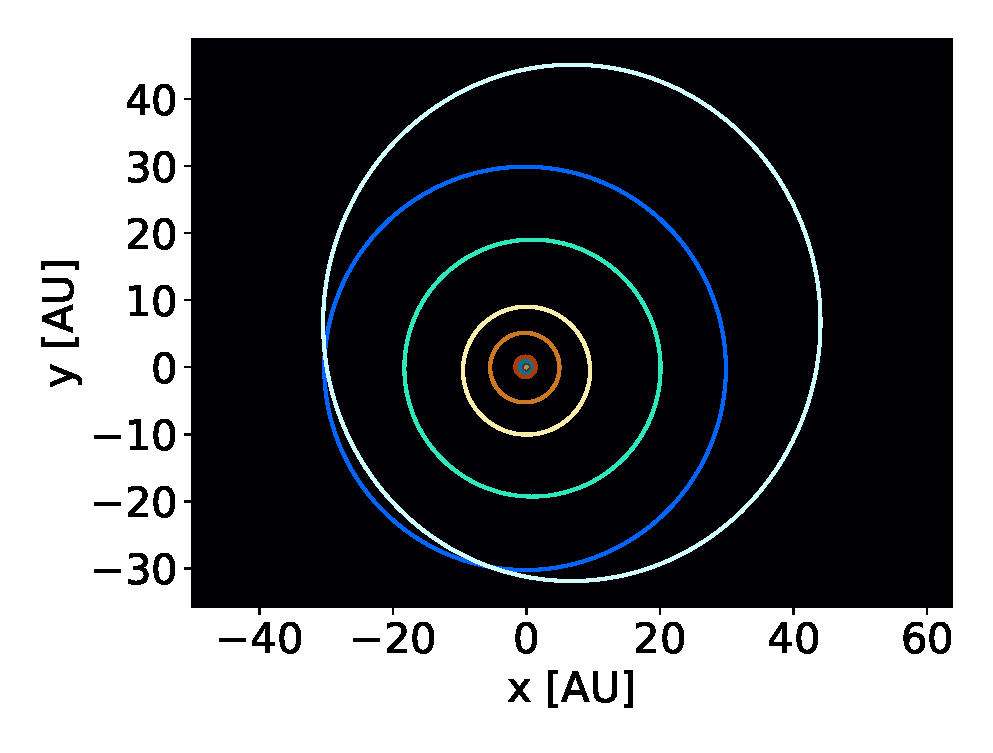
\includegraphics[width=\linewidth]{sol250vv72d.eps}
		\caption{2D plot in the $xy$-plane.}
	\end{subfigure}
	\caption{Plots in 3D and 2D of the planet orbits calculated over 250 years using $10^7$ time steps with the velocity Verlet method.}
	\label{fig:sol}
\end{figure*}
Figure \ref{fig:sol} shows  plots of the planet orbits calculated over 250 years using $10^7$ time steps with the velocity Verlet method. 

%Plots of the simulated solar system using the three algorithms are shown in figures \ref{fig:E}, \ref{fig:EC} and \ref{fig:vV}. With the Forward Euler algorithm, all planets spiral outwards, and \note{energy and angular momentum}.

We did not observe the expected effect of the relativistic correction on Mercury's orbit. When performing the simulation outside the class and noting the perihelion at each rotation, we observed an uneven oscillation, as shown in table \ref{tab:rel}.
\begin{table}[H]
	\centering
	\caption{The simulated perihelion angle in arc seconds with $10^8$ time steps over 1 year}
	\label{tab:rel}
	\begin{tabular}{|C|C|C|}\hline
	\text{time} & \text{no correction} & \text{correction} \\\hline
	0.240732 & -0.0216691 & -0.0411645	\\
	0.481463& 0.0399781 & 0.000987479	\\
	0.722195& 0.0180526 & -0.0404334	\\
	0.962927& -0.00400282 &  0.0014609	\\\hline
	\end{tabular}
\end{table}


%
%
%
\section*{Discussion}

We observed in figure \ref{fig:compare}, as expected, that the Forward Euler method causes the energy to increase and the angular momentum to decrease as the planets spiral outwards. The relative change is 67\% in energy and 70\% in angular momentum 
For the Euler-Cromer and velocity Verlet methods, the changes in energy and angular momentum are over ten orders of magnitude smaller then the values. This is small enough to be consistent with the expected conservation. 
The changes are still considerably smaller with the velocity Verlet method, showing that it is indeed more accurate.

In figure \ref{fig:esj} we see that while both the Earth and Jupiter were initialized to form circular orbits on their own, neither of them form perfect circular orbits in the three body system. As the mass of Jupiter increases, the radius of the Sun's orbit increases, and the Earth's orbit becomes elliptical with a perihelion precession. This is clearly visible in figure \ref{fig:esj10}. 
When the mass of Jupiter approximately equals that of the Sun (figure \ref{fig:esj1}), they form a binary system of rotation around the center of mass, while the Earth seems to move chaotically before it is ejected. 
In this case the program doesn't conserve energy. This likely happens as the Earth gets very close to the Sun at $(-0.5,1.5)$. The acceleration would be too large compared to the time step, resulting in the observed increase in energy.  

Over one year, we expect, for Mercury, to observe a perihelion precession of $0.45\un{\arcsecond}$ when the relativistic correction is applied. Instead we observe, with or without the correction, an oscillation with amplitude of the order $10^{-2}\un\arcsecond$. The relativistic correction seems to increase the amplitude slightly, but there is no indication of a consistent perihelion precession. 
We obtained similar behaviour when using a longer time or an increased correction, as well as when switching to the Euler-Cromer algorithm. 
We have not been able to identify the error. 

Simulating complete orbits of the outermost planets, and Pluto, requires a simulation time of multiple centuries. Since we use the same time steps for all planets, this results in inaccurate orbits for the inner planets with the number of time steps we are capable of simulating. 
In order to get accurate orbits for the inner planets, the simulation time must be reduced below ten years. 
This is a major weakness of the program, and potential solutions are discussed below.      

%After simulating for an integer number of years, we expect the Earth to be at approximately the same position, \note{compare ec and vv}


The accuracy of the  program is severely limited in the number of time steps which can be simulated. We present here some possible improvements.
The current program stores all positions and velocities within the PhysicsSimulator class, to be extracted after the simulation has been completed. In order to save memory and allow for simulations with more time steps, it would have been better to store only the values used by the class, and extract the values required by the main program at each step. This would remove memory as a limiting factor on the number of time steps.
Another improvement would be to employ adaptive methods. These adapt the time step to motion of the objects, resulting in consistent accuracy over the entire solar system.   

%
%
%
\section*{Conclusion}
The PhysicsSimulator class can simulate a system of multiple bodies interacting via classical gravity using the Euler, Euler-Cromer and velocity Verlet algorithms. 
Applying the program to a two body system showed that using Euler's method resulted in the bodies spiraling outwards, thus increasing energy and decreasing the angular momentum, with a relative change of 67\% and 70\%, respectively. 
The two other algorithms both conserve energy and angular momentum, and we confirmed that velocity Verlet is more accurate than Euler-Cromer.

Simulations of the three body system consisting og the Sun, Earth and Jupiter showed that Jupiter's influence on the Earth's orbit results noticeable perihelion precession. 

When simulating the entire solar system, the time required to get full orbits of the outermost planets meant our program lost the time resolution necessary to accurately simulate the innermost planets. We've outlined potential ways to fix this problem. The limit on the number of time steps can be removed by restructuring the data flow, and the time resolution for the inner planets can be improved by implementing adaptive methods.





\onecolumn
\begin{thebibliography}{9}

\bibitem{labtext}
Morten Hjorth-Jensen. Project 3. 2020. \textsc{url: }\url{http://compphysics.github.io/ComputationalPhysics/doc/Projects/2020/Project3/html/Project3.html}

\bibitem{lecture}
Morten Hjorth-Jensen. Computational Physics Lectures: Ordinary differential equations. 2020. \textsc{url: }\url{http://compphysics.github.io/ComputationalPhysics/doc/pub/ode/html/ode.html}


\end{thebibliography}



% Husk å avslutte alle environments
% SLUTT
\end{document}